%==============================================================================
%  Speech Communication full-length article (D59): the threshold-transfer audit, two registered rounds.
%  Round 1 = the registered audit as revised for the simulated ICME panel (DFV_Conference/revision, audited numbers).
%  Round 2 = PREREGISTRATION_ROUND2.md (tag round2-freeze). Every round-2 number comes from a generated table
%  (analysis/round2/r2_paper_tables.py -> gen/r2_*.tex) or carries a "% src:" comment; \todo{} marks what the authors
%  still have to supply. Checked by audit_claims.py. Supplement in supplement.tex; no venue page cap is imposed.
%==============================================================================
\documentclass[review,authoryear]{elsarticle}
\usepackage{amsmath,amssymb}
\usepackage{lmodern}
\usepackage{graphicx}
\graphicspath{{figures/}}
\usepackage{booktabs}
\usepackage{array}
\usepackage{hyperref}
\usepackage{xcolor}
\usepackage{url}
\usepackage{microtype}
\setlength{\emergencystretch}{2em}

\newcommand{\todo}[1]{\textcolor{red}{[#1]}}
\newcommand{\gentab}[1]{\IfFileExists{gen/#1.tex}{\input{gen/#1}}{\todo{generated table \detokenize{#1} pending}}}
\journal{Speech Communication}

\newcommand{\ttg}{\mathrm{TTG}}
\newcommand{\hter}{\mathrm{HTER}}
\newcommand{\frr}{\mathrm{FRR}}
\newcommand{\far}{\mathrm{FAR}}
\newcommand{\eer}{\mathrm{EER}}
\newcommand{\tauE}{\tau^{*}_{\mathrm{EER}}}
\newcommand{\tauF}[1]{\tau^{*}_{\mathrm{FRR}#1}}
\newcommand{\tauA}[1]{\tau^{*}_{\mathrm{FAR}#1}}

\begin{document}

\begin{frontmatter}
\title{Thresholded Once, Deployed Elsewhere: A Two-Round Pre-Registered Audit of Threshold Transfer in Speech Deepfake Detection}
\author{\todo{Author names}}
\address{\todo{Affiliations and corresponding-author email}}

\begin{abstract}
% src: revision/paper/main.tex; revision/results/b_thresholds.json; results/round2/analysis/r2_registered.txt; results/round2/analysis/r2_explore.txt
A speech deepfake detector's decision threshold is chosen on development data and then applied to speech from other
speakers, channels and synthesis systems. We propose a reporting protocol for this transfer and apply it in a two-round
pre-registered audit. The protocol splits the half total error rate at the development threshold into the error that no
threshold removes and a threshold transfer gap (TTG), reports false rejection and false acceptance under explicit
policies, and states the thresholds that tie on development data and speaker-level uncertainty. Round~1 audits five
released detectors trained on ASVspoof~2019 LA. On its unseen attacks, transfer causes 83--84\% of the deployed error of
two detectors whose equal error rates are below 1\%. On In-the-Wild, false rejection exceeds false acceptance for three
of four primary models when clips are resampled, as registered, but for one of four when speakers are resampled, so we
do not claim it; a neural codec raises false rejection more than false acceptance under both units. Two quantization
hypotheses were not supported, one for lack of usable quantized models and one on a clause the quantizer could not meet.
Round~2, registered before any of its scores existed, confirms that the operating policy sets the dominant error for
two of three current detectors and that the transfer gap recurs across retraining (four of five seeds). Trimming silence
from training lowers false rejection but not the equal error rate, largely through checkpoint selection. Low-bitrate
codecs and a phone impulse response raise false rejection more than false acceptance (four of eight channel conditions).
Detectors that discriminate In-the-Wild well remain limited by their thresholds, and review budgets designed on
development data do not survive transfer.
\end{abstract}

\begin{keyword}
speech deepfake detection \sep evaluation methodology \sep threshold transfer \sep calibration \sep domain shift
\end{keyword}
\end{frontmatter}

\section{Introduction}
\label{sec:intro}
Speech synthesis and voice conversion have made the assessment of speech authenticity an operational problem for
speech technology. A countermeasure (CM) produces a score, but a screening service or a moderation workflow must turn
that score into a decision. Its threshold is chosen using development data and then applied to speech whose speakers,
recording conditions and synthesis systems may differ from those used to choose it. Assessing this decision requires
more than a measure of how well the scores rank genuine and spoofed speech.

The equal error rate (EER) and minimum tandem detection cost are useful measures of discrimination
\citep{kinnunen18_tdcf,wang20_asvspoof2019,liu23_asvspoof2021}. They use evaluation labels to locate a favourable
operating point. A development threshold has no such access to the target labels. Consequently, a low evaluation EER
does not establish that a threshold selected elsewhere will preserve either the false-rejection budget for genuine
speech or the false-acceptance budget for spoofs. \citet{zhou26_eer_hides} demonstrate this distinction for a speech
deepfake detector transferred to In-the-Wild (ITW).

This distinction has a long history in biometric evaluation. Half total error rate (HTER) at a development threshold
is established practice in authentication and presentation-attack detection
\citep{bengio04_hter,chingovska12_lbp,korshunov16_crossdb}. Application-independent speaker-recognition evaluation
separates discrimination from calibration through actual and minimum detection costs
\citep{brummer06_calibration,vanleeuwen07_intro}. We apply that distinction to speech deepfake countermeasures. The
threshold transfer gap (TTG) is the excess target HTER at the source development threshold over the best HTER achievable
by thresholding the same target scores. It gives the threshold-dependent part of the error a separate name and
reports it beside the error that threshold selection cannot remove.

A threshold-transfer audit must also state whose errors it counts and how its operating point was chosen. Genuine
speech falsely rejected as spoofed may interrupt screening or prompt an incorrect authenticity accusation; a spoof
accepted as genuine may evade the same workflow. Their relative frequencies depend on the threshold policy, the
target distribution and the application costs. Furthermore, a development set with almost separated classes can
admit several nearly equivalent thresholds that behave differently after transfer. These are assessment questions,
even when the underlying detector architecture remains unchanged.

% src: PREREGISTRATION.md; PREREGISTRATION_ROUND2.md sections 1, 3, 4, 5.
We study these questions in two separately registered rounds. Round~1 audits five released checkpoints trained on the
ASVspoof~2019 logical-access data (LA19),
keeping their author-defined score and input conventions. Round~2 asks whether the findings extend to current
detectors, retrained AASIST-L models, the same recipe trained and evaluated on silence-trimmed speech, and additional
channel conditions. Its design was frozen after the round-1 findings were known and before any round-2 development
or target score existed. This chronology distinguishes replication on new scores from a claim that the later
hypotheses were formed without knowledge of the earlier audit.

The contribution is an assessment protocol and an empirical audit rather than a new detection architecture.
Table~\ref{tab:card} sets out the reporting protocol: development-only threshold selection, separate false-rejection
and false-acceptance rates, discrimination and transfer losses, development-threshold ambiguity, speaker-aware
uncertainty, and cost-sensitive interpretation. The audit distinguishes registered tests from exploratory
sensitivity analyses and examines whether its observations concern released checkpoints or a retrained recipe.
It also evaluates a development-designed accept/review/reject policy by the errors it automates and the traffic it
sends to review. The accompanying reproducibility package is described in the data-availability statement.

All detector scores in this article use desktop floating-point inference. The separate deployment study concerns
conversion, quantization and device measurements. The outcomes of the original quantization hypotheses are
disclosed here to preserve the registration record; their analyses belong to that separate study.

% Literature-only draft: no round-2 outcomes or empirical literature numbers.
% Primary-source verification is recorded beside the relevant bibliography entries.
\section{Related Work}
\label{sec:related}

\subsection{Threshold-aware evaluation in speech and biometrics}
% src: bib:bengio04_hter
The distinction between selecting a decision rule and evaluating it is established in biometric authentication.
\citet{bengio04_hter} evaluate HTER on a test set after selecting an EER threshold on separate validation data, and
show why uncertainty in the class-specific errors matters for statistical comparison. Face presentation-attack
detection also uses development-set thresholds followed by test-set HTER \citep{chingovska12_lbp}.
For speech, \citet{korshunov16_crossdb} use the same separation when transferring countermeasures between databases
and between logical-access and replay attacks. These precedents motivate keeping the threshold-selection data
explicit when assessing a speech deepfake detector.

% src: bib:brummer06_calibration
Speaker-recognition evaluation further distinguishes discrimination, described by the attainable error trade-offs,
from calibration, which determines how well a score supports a particular decision rule
\citep{brummer06_calibration,vanleeuwen07_intro}. The difference between actual cost and minimum cost expresses this
distinction for a specified application. A minimum found using evaluation labels describes what an oracle threshold
could achieve; actual cost evaluates the supplied scores at the application's threshold. Our TTG follows this
lineage at the equal-cost operating point: it measures the excess HTER of a development threshold above the target's
minimum HTER. It is a threshold-specific loss, rather than a claim that the CM scores are calibrated likelihood
ratios across applications.

% src: bib:wang20_asvspoof2019
The ASVspoof challenges provide a complementary evaluation lineage. ASVspoof~2019 and ASVspoof~2021 report EER and
minimum tandem detection cost, with t-DCF assessing a countermeasure together with an ASV system; the 2021 deepfake
(DF) track, which involves no ASV system, reports EER only \citep{kinnunen18_tdcf,wang20_asvspoof2019,liu23_asvspoof2021}. The stand-alone detection track of ASVspoof~5 reports
minimum DCF, actual DCF, and log-likelihood-ratio cost \citep{wang24_asvspoof5}. Its actual DCF uses a fixed Bayes
threshold under an LLR interpretation of the submitted scores. This differs from transferring an empirical
development threshold, but both protocols expose behavior that a threshold optimized on the target cannot reveal.

% src: bib:zhou26_eer_hides
A direct speech-deepfake precedent is \citet{zhou26_eer_hides}, who freeze an SSL-AASIST detector, select a source
EER threshold on labelled ASVspoof~2019 LA evaluation data, and transfer it to In-the-Wild and a subset of
ASVspoof~2021 DF. They report HTER and its false-rejection/false-acceptance decomposition, and audit unlabelled
score corrections. Their monotone-invariance argument clarifies that a strictly increasing score transform can
alter decisions at a fixed numerical threshold while leaving the ROC and EER unchanged. Our audit uses development data for
threshold selection and extends the assessment across checkpoints, policies, training runs, and controlled
perturbations. The contribution is the scope and registration of this assessment, rather than the invention of
transferred-threshold evaluation.

\subsection{Generalization, dataset cues, and training variability}
% src: bib:muller22_in_the_wild
Cross-corpus evaluation tests more than the ability to reject a new synthesis algorithm. In-the-Wild collects
authentic and manipulated speech of public figures from online media, and demonstrates poor generalization of
ASVspoof-trained detectors to that setting \citep{muller22_in_the_wild}. Recording conditions, speech content,
speakers, and generation pipelines can change together. A target EER summarizes the resulting discrimination,
whereas the transferred FRR and FAR additionally reveal which class a deployed rule harms.

% src: bib:muller21_silence
Dataset cues can make this distinction harder to interpret. \citet{muller21_silence} identify label-correlated
leading and trailing silence in ASVspoof data; silence-duration classifiers are predictive, and training established
CMs after trimming silence changes their detection performance. Their evidence motivates interventions on the
training audio, rather than treating a test-time trim alone as evidence that a detector has learned a particular
causal mechanism. Our paired training design asks whether removing this cue changes the transferred operating
behavior, with source performance serving as a manipulation check.

% src: bib:wang25_asvspoof5_db
ASVspoof~5 explicitly addresses collection artefacts. Its shortcut-reduction pipeline normalizes peak amplitude,
randomly trims leading and trailing non-speech, and varies the retained utterance duration. The database paper
states that this pipeline is applied to the development and evaluation sets, but not the training set
\citep{wang25_asvspoof5_db}. Consequently, a detector trained on that release is not automatically trained on
shortcut-reduced audio. Training variability is another source of uncertainty:
\citet{wang21_comparative} show that changing initialization can produce statistically distinguishable performance
for the same CM recipe. Replication over training runs therefore complements comparisons of released checkpoints.

\subsection{Countermeasure architectures and probability calibration}
% src: bib:tak21_rawnet2
The checkpoints in this audit span distinct representation choices. RawNet2 learns directly from waveforms
\citep{tak21_rawnet2}, while Res-TSSDNet uses a residual time-domain network \citep{hua21_res_tssdnet}.
AASIST integrates spectral and temporal graph-attention representations, and AASIST-L is its lighter variant
\citep{jung22_aasist}. These models support an assessment across architectures without attributing every difference
in transfer behavior to a single back end.

% src: bib:tak22_xlsr_aasist
Self-supervised speech representations broaden the feature space available to CMs. \citet{tak22_xlsr_aasist}
combine a wav2vec~2.0 front end with an AASIST back end and data augmentation. XLS-R supplies multilingual pretrained
speech representations \citep{babu21_xlsr}; XLSR-Mamba combines that representation family with a dual-column
bidirectional state-space back end \citep{xiao25_xlsrmamba}. Improvements in discrimination under these designs do
not themselves establish that a source decision threshold will transfer.

% src: bib:pascu24_calibrated
\citet{pascu24_calibrated} address both generalization and prediction reliability using frozen self-supervised
representations with logistic regression. They assess discrimination with EER and probability calibration with
expected calibration error. ECE describes agreement between predicted probabilities and observed class frequencies
within probability bins; it does not evaluate a particular source threshold after transfer. Including a detector designed
with this calibration objective allows the audit to examine that distinction empirically, without presuming that
probability calibration removes operating-point drift.

\subsection{Channel, codec, and multilingual shift}
% src: bib:liu23_asvspoof2021
Communication processing can alter detection cues in both genuine and manipulated speech. ASVspoof~2021 DF
includes media compression, while ASVspoof~5 applies encoding and compression, including EnCodec, to evaluation
utterances from both classes \citep{liu23_asvspoof2021,wang25_asvspoof5_db}. The communication benchmark of
\citet{realworld_comms24} investigates combinations of codecs and packet loss. These studies motivate controlling
channel changes when comparing clean and perturbed scores, and reporting the class-specific errors of the
transferred rule in addition to threshold-optimized detection performance.

% src: bib:wu24_codecfake
Neural codecs also participate in speech generation. CodecFake trains countermeasures on codec-resynthesized
speech to improve detection of codec-based synthesis \citep{wu24_codecfake}.
\citet{xiao26_resynth} examine the resulting label ambiguity: a codec can be either a transmission mechanism or
part of a synthesis pipeline. The codec operation alone therefore does not specify the audit's target label.
Our channel stress tests preserve the clean utterance's label and state that assumption explicitly; this assesses
the treatment of genuine speech carried through a channel, rather than defining every resynthesis as an attack.

% src: bib:mlaad24
MLAAD expands evaluation beyond predominantly English benchmarks by providing synthetic speech across languages
and synthesis architectures \citep{mlaad24}. Its distributed audio is synthetic; corresponding original human
recordings are supplied by the M-AILABS source corpus \citep{solak17_mailabs}. This distinction matters for threshold auditing: spoof-only
data can measure attack acceptance at a frozen threshold, but cannot identify false rejection or a complete HTER.
Language and synthesis coverage should therefore be reported separately from evidence about the operating rule on
bona fide traffic. The audit fixes the dataset version and pairing protocol in its study design.

\subsection{Selective decisions and transferred review policies}
% src: bib:geifman17_selective
Selective classification adds an abstention option, trading automatic-decision coverage for lower error among
the retained decisions \citep{geifman17_selective}. In speech screening, the abstention can become a review queue,
with acceptance and rejection on either side of a score band. A band chosen on development data remains a
transferred policy: its target review share and residual errors depend on the target score distribution. Our
three-zone assessment consequently measures coverage and class-specific automatic errors together. It does not
treat a source review budget as a guarantee of target workload, nor assume that a target-fitted oracle policy is
available during deployment.


% ============================ III. PROTOCOL =====================================
\section{Protocol}
\label{sec:protocol}

% src: PREREGISTRATION_ROUND2.md sections 6, 9; deploybench/metrics.py; revision/results/b_thresholds.json
\begin{table}[!t]
\caption{Reporting card for a threshold-transfer audit. The study's actual registration and deviation chronology is given in Section~\ref{sec:design}.}
\label{tab:card}
\centering
\footnotesize
\setlength{\tabcolsep}{3pt}
\begin{tabular}{@{}p{0.21\columnwidth}p{0.73\columnwidth}@{}}
\toprule
\emph{Inputs} & A CM that outputs a score; labelled source development data; target sets with speaker labels; one or more cost
models. \\
\emph{Specify before a new audit} & Threshold policies computed from development scores alone (EER; FRR budgets 1\% and
5\%; FAR budgets 1\% and 5\%), the estimator and its tie rule, the hypotheses and the resampling unit (speaker). \\
\emph{Report at each policy and target} & FRR (BPCER) and FAR (APCER) at the shipped threshold; HTER split into oracle HTER
and TTG, with speaker-level intervals; FRR and FAR at both ends of the interval of thresholds that tie on dev data; cost over
a sweep of priors, with its break-even window; the data and policy that set the threshold. \\
\emph{For triage} & The review share and the automatic-decision errors of a three-zone policy designed on dev data. \\
\bottomrule
\end{tabular}
\end{table}

% src: deploybench/metrics.py; PREREGISTRATION_ROUND2.md sections 6, 9; revision/results/b_thresholds.json; revision/results/e_cost.json
\subsection{Scores, thresholds and measures}
Each CM maps a clip \(x\) to a score \(s(x)\), higher meaning more bona fide, and declares a spoof if \(s(x)<\tau\). Every
threshold is fixed on the source development set of the model's training data. \(\tauE\) is the crossing of dev FRR and
FAR, estimated by linear interpolation between adjacent unique dev scores. \(\tauF{1}\) and \(\tauF{5}\) are the strictest
thresholds whose dev FRR stays within 1\% and 5\%, and \(\tauA{1}\) and \(\tauA{5}\) the most lenient thresholds whose dev
FAR stays within 1\% and 5\%, which correspond to BPCER at a fixed APCER in ISO/IEC 30107-3 terms \citep{iso30107_3}. On a target, \(\frr(\tau)\) is the share of
bona fide clips declared spoof (BPCER), \(\far(\tau)\) the share of spoofs accepted (APCER), and
\(\hter(\tau)=\tfrac12[\frr(\tau)+\far(\tau)]\) \citep{bengio04_hter}. For a transferred threshold \(\tau^{*}\),
\begin{equation}
\ttg(\tau^{*}) \;=\; \hter(\tau^{*}) \;-\; \min_{\tau}\hter(\tau)
\label{eq:ttg}
\end{equation}
is the calibration loss of \(\tau^{*}\) at the equal-cost point \citep{brummer06_calibration,vanleeuwen07_intro}. The
minimum, the oracle HTER, is the part of the deployed error that no threshold on these scores removes (discrimination), and TTG the
part that a better threshold would remove (transfer). We report both, and the transfer share \(\ttg/\hter(\tau^{*})\).
Because a near-separable development set pins \(\tauE\) with few trials, we also report the \emph{dev-equivalent
interval}: the connected run of thresholds around \(\tauE\) whose dev HTER exceeds \(\hter(\tauE)\) by at most one bona
fide trial (\(0.5/n_{\mathrm{bona}}\)), and the target FRR at its two ends.

% src: deploybench/metrics.py; PREREGISTRATION_ROUND2.md sections 6, 9; revision/results/b_thresholds.json; revision/results/e_cost.json
\emph{Cost.}\label{eq:cost} With \(p\) the bona fide prior weighted by costs, \(C(p,\tau)=[p\,\frr(\tau)+(1-p)\,\far(\tau)]/\min(p,1-p)\)
is 1 for the better trivial system, so a detector beats both trivial systems only for priors in
\(\far/(\far+1-\frr)<p<(1-\far)/(1-\far+\frr)\), its break-even window.

% src: PREREGISTRATION_ROUND2.md section 9 E7
\emph{Three-zone policy.} The registered extension uses a review band \([\tau_{\mathrm{lo}},\tau_{\mathrm{hi}})\) holding 10\% of the pooled dev scores,
centred in rank on \(\tauE\), sends scores inside it to review, rejects below it and accepts above it. On each target we
report the review share and the automatic errors, and compare with the same rule fitted to the labelled target and with a
label-free variant whose edges are re-anchored on the target's unlabelled scores.

% src: PREREGISTRATION.md; revision/results/b_thresholds.json; revision/paper/main.tex
% ============================ IV. STUDY DESIGN =====================================
\section{Study Design}
\label{sec:design}
\subsection{Round 1: released LA19-trained checkpoints}
% src: the ICME revision (DFV_Conference/revision/paper/main.tex Sec. III-B/C; audited by audit_claims.py).
Round~1 audits five published CMs: four primary models (AASIST and AASIST-L \citep{jung22_aasist}, RawNet2
\citep{tak21_rawnet2}, Res-TSSDNet \citep{hua21_res_tssdnet}) and a self-supervised reference, XLS-R+AASIST
\citep{tak22_xlsr_aasist} (Table~\ref{tab:roster}). Checkpoints are used as released; we vendor each author's code and keep
its score function, class order and input policy. A primary model must reproduce its published LA19 evaluation EER within
15\% (relative); the released RawNet2 is the ASVspoof~2021 DF baseline and is gated on DF21 against the organisers'
released scores (per-trial agreement \(3.7{\times}10^{-5}\)); XLS-R+AASIST has no published LA19 figure and enters no
hypothesis count. Every threshold is fixed on the LA19 development set (24,844 trials, 2,548 bona fide).

% src: revision/paper/gen/tab_roster.tex; revision/results/b_thresholds.json
\begin{table}[!t]
\caption{Round-1 roster and development thresholds. EER on LA19 eval (\%): ours / published. Dev EER (\%) and \(\tauE\) on
LA19 dev. Last column: dev bona fide trials below, and dev spoof trials at or above, \(\tauE\).}
\label{tab:roster}
\centering
\footnotesize
\setlength{\tabcolsep}{3pt}
\begin{tabular}{@{}lrcrrc@{}}
\toprule
Model & Params & Eval EER & Dev EER & $\tauE$ & Dev trials \\
\midrule
AASIST & 298K & 0.83 / 0.83 & 0.510 & $-$1.09 & 13 / 113 \\
AASIST-L & 85K & 0.99 / 0.99 & 0.510 & $-$0.94 & 13 / 113 \\
RawNet2 & 17.6M & 4.60 / 5.64\textsuperscript{a} & 0.549 & $-$7.07 & 14 / 122 \\
Res-TSSDNet & 349K & 1.62 / 1.66 & 0.722 & $-$8.24 & 19 / 161 \\
XLS-R (ref.) & 315M & 0.15 / ---\textsuperscript{b} & 0.009 & $-$1.75 & 1 / 2 \\
\bottomrule
\end{tabular}
\\[2pt]
\parbox{\columnwidth}{\footnotesize\textsuperscript{a}Different training run, gated on DF21 instead.
\textsuperscript{b}None published, so ungated and outside every hypothesis count.}
\end{table}

% src: PREREGISTRATION.md; DEVIATIONS.md DEV-2 and DEV-8; revision/results/g_docs.json; revision/paper/main.tex
The targets \citep{wang20_asvspoof2019,muller22_in_the_wild,liu23_asvspoof2021} are the LA19 evaluation set (71,237 trials; 11 of 13 attacks unseen), In-the-Wild (31,779 clips of public
figures with 54 distinct speaker labels in its metadata), a verified subset of ASVspoof~2021 DF (455,508 trials; libFLAC~1.4
rejects 43\% of the public evaluation files and for 78,420 of them the only working decode fails the file's own MD5, so we
exclude those), and an EnCodec stress set: 1,000 LA19-eval clips (500 per class, all 67 speakers) resynthesised at 6\,kbps
\citep{defossez23_encodec}, whose bona fide clips stay bona fide (a genuine user's speech through a codec is still
genuine) \citep{wang25_asvspoof5_db,xiao26_resynth}. The registered hypotheses were H2 (on ITW at \(\tauE\), FRR exceeds FAR
for at least three of the four primary models) and H5 (EnCodec raises FRR more than FAR, relative to the clean copy, for
at least three), tested by one-sided class-stratified bootstraps (B = 1,000) with Holm correction; because clips are nested
in speakers, we added speaker-cluster bootstraps (B = 10,000) as a logged, exploratory deviation \citep{bolle04_subsets,field07_boot}. The resampling unit for H2 was specified after the descriptive ITW rates had been seen. H1 and H4 are exploratory and receive effect sizes and intervals rather than confirm/refute claims; their detailed results appear in the supplement.
The hypotheses were registered on 19~July 2026, amended in August and September, and frozen on 28~September 2026 before any
ITW clip was scored; the frozen registration and the deviation log are in the repository. Two int8 hypotheses were also
registered; neither was supported (H3 for lack of usable int8 models, H6 on a clause the quantizer could never meet), and the separate deployment study will report their analyses.

% src: PREREGISTRATION_ROUND2.md § 1. Purpose and relation to round 1; § 2. What had been seen when this was written; DEVIATIONS.md DEV-9.
\subsection{Round 2: registered extension}
\label{sec:r2design}
Round~2 tests the scope of the released-checkpoint findings through detector changes, retraining,
a silence-removal intervention and additional channel conditions. The registration and analysis code were
frozen together at \texttt{round2-freeze}, before any round-2 development, evaluation or target score existed.
The design was informed by the completed round-1 analyses and published detector results; pre-freeze
score-pipeline smoke tests used LA19 training clips only. No audio for the additional stress conditions
had been generated. The round-1 roster, hypotheses and results remain fixed. The extension has its own
confirmatory families and descriptive reading rule; it does not add models to any round-1 hypothesis count.

\subsubsection{Detectors and evaluation surfaces}
% src: PREREGISTRATION_ROUND2.md § 3. Models; § 5. Data and targets.
The extension adds the ASVspoof~5 baseline AASIST, the logistic-regression detector of
\citet{pascu24_calibrated}, and XLSR-Mamba \citep{xiao25_xlsrmamba}. The first uses the released ASVspoof~5
checkpoint, trained on the training partition without the post-processing applied to the development and
evaluation partitions \citep{wang25_asvspoof5_db}. Pascu's detector uses frozen XLS-R~2B features
\citep{babu21_xlsr}, mean-pools the last hidden state and fits a logistic-regression head. We refit that head
on LA19 train alone, reserving LA19 dev for threshold setting; a separate train-plus-dev fit is used only
for the reproduction gate. XLSR-Mamba uses the released deepfake-detection checkpoint trained on LA19
with RawBoost augmentation \citep{tak22_rawboost}. Table~\ref{tab:r2matrix} gives the registered scoring
matrix and source of each model's thresholds.

% src: PREREGISTRATION_ROUND2.md § 3. Models; § 5. Data and targets; § 9. Exploratory analyses (E3, E6, E11).
\begin{table}[!t]
\caption{Registered round-2 model--surface matrix. LA19 eval and ITW are common targets; additional
targets are restricted as shown. ``Stress'' denotes the common clean manifest and channel variants.
The gate-only fit contributes no threshold-transfer result.}
\label{tab:r2matrix}
\centering
\footnotesize
\setlength{\tabcolsep}{4pt}
\begin{tabular}{@{}p{0.22\textwidth}p{0.20\textwidth}p{0.23\textwidth}p{0.27\textwidth}@{}}
\toprule
Model & Threshold source & Common targets & Additional targets \\
\midrule
ASVspoof~5 AASIST & ASVspoof~5 dev & LA19 eval, ITW, stress & Verified DF21, MLAAD-5, ASVspoof~5 eval \\
Pascu LR, train-only fit & LA19 dev & LA19 eval, ITW, stress & Verified DF21, MLAAD-5 \\
XLSR-Mamba & LA19 dev & LA19 eval, ITW, stress & Verified DF21, MLAAD-5 \\
AASIST-L, untrimmed runs & Each run's LA19 dev & LA19 eval, ITW, stress & None \\
AASIST-L, trimmed runs & Each run's trimmed LA19 dev & LA19 eval, ITW, stress & None \\
Last-epoch copies of both arms & Corresponding source dev & LA19 eval, ITW & None; selection-free analysis only \\
Pascu LR, train-plus-dev fit & None & LA19 eval for the gate & None \\
\bottomrule
\end{tabular}
\end{table}

% src: PREREGISTRATION_ROUND2.md § 3. Models; § 6. Scoring, gates and thresholds.
All scoring uses desktop fp32 arithmetic with TF32 disabled and the shared score convention of
Section~\ref{sec:protocol}. The ASVspoof~5 baseline and the AASIST-L runs use 64,600 samples;
XLSR-Mamba uses 66,800 samples on every surface, including ITW. Evaluation retains the start of long
clips and repeat-tiles short clips according to the author implementations. Pascu's detector uses
the whole utterance; its score is the bona fide log-odds, obtained by reversing the sign of the fitted
classifier's fake-class decision function. These input and score rules are fixed across targets.

% src: PREREGISTRATION_ROUND2.md § 6. Scoring, gates and thresholds; § 10. Failure, missing data and stopping rules.
The reproduction gates check pipeline fidelity, rather than transfer performance. The ASVspoof~5
baseline must reproduce its published development EER within 15\% relative error. XLSR-Mamba is
compared with the authors' released deepfake scores on the same verified DF21 trials and at the same
input length, using the same relative tolerance. Pascu's separate train-plus-dev fit must reproduce
the published LA19-eval EER within that tolerance; it is reported only as a gate, not as an audited
detector. The training runs have no reproduction gate. A gate failure remains visible in exploratory
reporting and counts against support of the detector hypothesis; it does not trigger checkpoint or
model substitution. Every operational model receives all five registered policies from its own source
dev: \(\tauE\), \(\tauF{1}\), \(\tauF{5}\), \(\tauA{1}\) and \(\tauA{5}\). Those thresholds are frozen
once written, with no target-dependent tuning.

\subsubsection{Retraining and the silence intervention}
% src: PREREGISTRATION_ROUND2.md § 3. Models; § 4. Training runs.
We retrain the author's AASIST-L recipe \citep{jung22_aasist} with seeds 1--5 in each of two arms:
the original audio and audio trimmed by the fixed energy-VAD rule. An additional untrimmed run at the
author's default seed, 1234, checks the pipeline and enters the exploratory seed comparison only.
The schedule is held fixed: 100 epochs, batches of 24, Adam with an initial learning rate of
\(10^{-4}\), per-step cosine annealing to \(5\times10^{-6}\), weight decay \(10^{-4}\), and the recipe's
class-weighted cross-entropy. Evaluation data are excluded from training and checkpoint selection;
the author's evaluation-based best-checkpoint step is omitted.

% src: PREREGISTRATION_ROUND2.md § 4. Training runs.
The primary checkpoint is the recipe's final stochastic weight average (\texttt{swa.pth}). The
selection rule is preserved, including its initial incumbent dev EER of 1 on a percentage scale:
only epochs selected by the dev-improvement rule at an EER no greater than 1\% can enter the average.
If none is selected, the primary checkpoint is the last epoch. We report the number of snapshots
contributing to each average. The initial incumbent is a selection state, not an observed minimum
dev EER; the latter must be taken from the epoch log. Last-epoch weights are saved separately for
the selection-free comparison, and are identical to the primary weights when the average has no
snapshots. This comparison tests whether any difference between arms depends on dev-based
checkpoint selection.

% src: PREREGISTRATION_ROUND2.md § 4. Training runs (trimmed arm); § 10. Failure, missing data and stopping rules.
The VAD computes frame energy from float32 samples with 25-ms frames and a 10-ms hop. Frames within
35~dB of the clip's loudest frame are active. Both ends are cut with no added margin; a clip is left
untrimmed if the retained region would be shorter than 0.25~s. In the trimmed arm, this operation
precedes the recipe's random training crop or evaluation padding on train and dev, and precedes
padding for every scored input. Thus the intervention changes the full training-and-scoring pipeline
while keeping the detector recipe fixed. The comparison concerns this recipe and this explicit
silence rule. A pre-training check refuses any trimmed training clip of exactly 64,600 samples,
which would otherwise hit the recipe's undefined random-crop boundary.

\subsubsection{Channel intervention}
% src: PREREGISTRATION_ROUND2.md § 5. Data and targets.
The channel experiment uses the frozen, class-balanced 1,000-clip LA19-eval manifest from H5 and a
byte-identical clean copy. It adds Opus at 6 and 24~kbps, AMR-NB at 4.75~kbps, MP3 at 32~kbps,
MUSAN noise \citep{snyder15_musan} at 20, 10 and 5~dB SNR, and a mock-up-phone impulse response
from AIR within RIRS\_NOISES \citep{jeub09_air,ko17_rirs}. Codec outputs are decoded to 16-kHz PCM;
AMR-NB coding uses 8~kHz internally. Noise-file selection and offset are deterministic functions of
the utterance identifier, and SNR is defined over the whole clip. The impulse response is chosen in
the same deterministic way, its channels are averaged to mono and the response is peak-normalised
before convolution. The output is cut to the input length and peak-limited if needed to avoid clipping.
A response at an incompatible sample rate is refused,
and the chosen files and hashes are retained as provenance. The existing EnCodec condition is kept
for exploratory comparison. Every round-1 model, round-2 detector and primary training-run checkpoint
is scored on the stress set; last-epoch copies are excluded. These are channel perturbations of the
same labelled clips, so bona fide labels are retained.

\subsubsection{Confirmatory tests and their reading}
% src: PREREGISTRATION_ROUND2.md § 5. Data and targets; § 7. Confirmatory hypotheses (common rules).
For target-level tests, speakers are resampled with replacement and all their clips of both classes
are retained. ITW uses its supplied speaker labels and LA19 eval uses its corpus speakers. Each
bootstrap test uses \(B=10{,}000\), seed 0, and the registered one-sided probability
\(p=(1+\#\{T_b\leq0\})/(B+1)\), with the tested statistic centred at the null boundary.
Holm's procedure controls \(\alpha=0.05\) within each specified family \citep{holm79_holm}.
The following definitions fix the support rules and interpretation before outcomes are read.

\begin{description}
% src: PREREGISTRATION_ROUND2.md § 7. Confirmatory hypotheses (R2-H1).
\item[R2-H1: policy and error direction.]
For each new detector on ITW, test \(\frr-\far>0\) at \(\tauF{1}\), and
\(\far-\frr>0\) at \(\tauA{5}\). Holm correction covers all six tests. A detector supports the
hypothesis only when both nulls are rejected; overall support requires at least two of the three
detectors. A failed gate or an unscorable detector counts as not supporting it. Failure of the
overall rule means that transferred error direction depends on the detector as well as the policy.

% src: PREREGISTRATION_ROUND2.md § 7. Confirmatory hypotheses (R2-H2).
\item[R2-H2: transfer gap across retraining.]
For each untrimmed AASIST-L run, test whether LA19-eval TTG at \(\tauE\) exceeds 1~pp,
recomputing the oracle HTER in every speaker-cluster replicate. Holm correction covers the five
runs, and support requires at least four rejections. A missing run counts as not rejecting.
Support would extend the released-checkpoint transfer-gap finding to repeated training of this
recipe at the registered margin.

% src: PREREGISTRATION_ROUND2.md § 7. Confirmatory hypotheses (R2-H3).
\item[R2-H3: training without the silence cue.]
Compare the trimmed and untrimmed run means using exact one-sided permutation tests over the 252
reassignments under the full planned five-per-arm design; with eligible missing runs, enumerate the assignments
of the remaining run counts. Higher trimmed-arm LA19-dev EER is the manipulation check,
outside the correction family. The family contains lower ITW FRR at \(\tauE\) and lower ITW EER in
the trimmed arm. Rejection for FRR alone indicates an operating-point effect; rejection for both FRR and EER indicates
an additional effect on discrimination. If neither null is rejected, the registered reading
is that the intervention does not explain the recipe's ITW behaviour. With fewer than three completed runs in either arm, the hypothesis is
not evaluable; the registered analysis uses the remaining runs when that minimum is met.

% src: PREREGISTRATION_ROUND2.md § 7. Confirmatory hypotheses (R2-H4).
\item[R2-H4: additional channels.]
For each new condition and each primary round-1 model, test
\(\Delta\frr-\Delta\far>0\) at the frozen round-1 \(\tauE\), relative to the clean copy of the
same clips. Clean and stressed scores remain paired in speaker resampling. Holm correction covers
the four models within each condition, and a condition supports the hypothesis if at least three
models reject. The component tests \(\Delta\frr>0\) and \(\Delta\far<0\) are corrected and
reported in the same way. Reporting is by condition, including the number of conditions meeting
the rule, rather than a pooled claim across channels.
\end{description}

% src: PREREGISTRATION_ROUND2.md § 8. Reading rule R2-RL (fixed in advance, descriptive).
The descriptive reading rule applies to each new detector on ITW at \(\tauE\) in a fixed order.
An ITW EER of at least 20\% is \emph{discrimination-limited}. Otherwise, a detector is
\emph{transfer-limited} if its TTG/HTER is at least 0.5 or its source-dev-equivalent threshold
interval spans at least 10~pp of ITW FRR. It is \emph{well-transferred} if the share is below 0.2
and the span below 5~pp, and \emph{intermediate} otherwise. These categories describe whether the
round-1 pattern carries over; they are not additional hypothesis tests.

\subsubsection{Exploratory analyses}
% src: PREREGISTRATION_ROUND2.md § 9. Exploratory analyses (E1--E6).
The exploratory programme reports effect sizes and intervals without confirmatory language.
E1 describes FRR, FAR, HTER, oracle HTER, TTG, transfer share, dev-equivalent intervals and their
target endpoints, and the rank-based miss and band on every registered model--surface--policy cell,
using speaker-cluster 95\% intervals with \(B=1{,}000\). E2 places the released AASIST-L values
within the spread of the retrained arms, including the pipeline-check run. E3 compares last-epoch
copies without checkpoint selection, and E4 reports paired channel effects for every scored model
and run, including EnCodec. E5 reports the new detectors on MLAAD-5 by language and states its
sample-rate confound with every numerical result: native sample rate is associated with class,
as quantified by the round-1 census in Table~\ref{tab:r1mlaad}. The already-seen round-1 MLAAD results remain descriptive. E6 reports
the ASVspoof~5 baseline by evaluation condition, with codec-free C00 primary, and characterises
development and evaluation silence with the same VAD.

% src: PREREGISTRATION_ROUND2.md § 9. Exploratory analyses (E7, E8).
E7 evaluates development-designed accept/review/reject policies. The primary review budget is
10\% of pooled dev traffic, centred in rank at \(\tauE\), with edges at
\(F_{\mathrm{dev}}(\tauE)\pm0.05\). Each target contributes its pooled and class-specific review
shares, bona fide auto-rejection and spoof auto-acceptance. Comparators use the same construction
at the labelled target oracle and a label-free variant re-anchored on the target's pooled scores.
Secondary budgets are 5\% and 20\%. A separate error-budget rule rejects below \(\tauF{1}\) and
accepts from \(\tauA{1}\); if those bounds cross or coincide, it collapses to \(\tauE\), and the
collapse is reported. E8 gives the APCER/FAR and BPCER/FRR reading at every policy, including
BPCER at source-fixed APCER budgets of 1\% and 5\% and at the corresponding target oracle.

% src: PREREGISTRATION_ROUND2.md § 9. Exploratory analyses (E9--E11); DEVIATIONS.md DEV-9 amendment 2.
E9 compares actual and minimum normalised cost after an unpenalised logistic calibration fitted
on source dev alone, with prior correction and Bayes thresholds over logit priors from \(-4\) to
\(4\) in steps of 0.25. The logged amendment replaces the registered fixed-step fitting routine
with the maximum-likelihood logistic fit after a unit test exposed scale-dependent underfitting;
the prior sweep and cost comparison are unchanged. E10 reports the screening and forensic
break-even windows at \(\tauE\), using the round-1 cost models. E11 contains the train-plus-dev
Pascu fit solely as the reproduction gate.

\subsubsection{Failures and amendments}
% src: PREREGISTRATION_ROUND2.md § 10. Failure, missing data and stopping rules; DEVIATIONS.md DEV-9 amendment 1.
The failure rules prohibit replacement detectors, additional seeds and repetition after training
divergence, NaN loss or a training crash. Missing runs count against the registered retraining
support rule; the silence test uses only the completed runs subject to its evaluability minimum.
A logged resource amendment permits a run that fails before completing its first epoch, before
any dev score exists, to restart once from scratch with the same seed, code and data. Scheduling
was adjusted using observed memory requirements, with failed directories retained. This exception
does not permit restarting a run after training outcomes have been observed. A logistic-regression
convergence warning is reported and the fitted head is retained.

% src: PREREGISTRATION_ROUND2.md § 10. Failure, missing data and stopping rules; DEVIATIONS.md DEV-9 amendment 3.
Loaders refuse unknown labels or codecs, incorrect row counts and missing files. Every such fix
is logged before rerunning the affected job. The FLAC amendment requires native or fallback
integer decoding to match the file's STREAMINFO MD5 before explicit float32 conversion. It was
logged after a decoder sign error was found, before any affected round-2 DF21 score was analysed;
the affected scores were quarantined for re-scoring. This preserves the registered verified
surface and prevents an environment-specific decoder from silently changing its audio.

% src: DEVIATIONS.md DEV-9 amendment 4.
A separate amendment permits one unchanged rerun of Pascu's whole-utterance MLAAD-5 scoring on a
GPU free of a training run, with an expandable memory-allocator setting. It does not shorten
utterances, change the head or alter arithmetic. A second failure is reported as missing MLAAD-5
data; that surface contributes only to the exploratory language analysis. Each amendment records
what had been seen when it was made. These resource and fidelity amendments are reported alongside
the frozen design, rather than used to revise its tests or support thresholds.


% src: revision/paper/gen/tab_operating.tex; revision/results/a_cluster.json
% ============================ V. RESULTS: ROUND 1 ======================================
\section{Round 1: Released Checkpoints}
\label{sec:round1}
% src: the ICME revision Sec. IV (results/b_thresholds.txt, a_cluster.txt, f_vad_*.txt, a5_cheapcheck.txt, e_cost.txt).
\begin{table*}[!t]
\caption{Round 1: operating behaviour at the frozen \(\tauE\) (fp32, \%). HTER = oracle HTER (discrimination) + TTG
(transfer, pp); TTG/HTER is the transfer share (\%). The CI of TTG is a speaker-cluster bootstrap (B = 1,000).}
\label{tab:op}
\centering
\footnotesize
\setlength{\tabcolsep}{5pt}
\resizebox{\textwidth}{!}{\begin{tabular}{@{}lrrrrrrlr@{}}
\toprule
Model & EER & FRR & FAR & HTER & Oracle & TTG & 95\% CI (speaker bootstrap) & TTG/HTER \\
\midrule
\multicolumn{9}{@{}l}{\emph{LA19 eval: seen corpus, unseen attacks} (67 speakers)} \\
AASIST & 0.83 & 0.16 & 9.83 & 5.00 & 0.82 & 4.18 & [3.74, 4.65] & 84 \\
AASIST-L & 0.99 & 0.10 & 11.14 & 5.62 & 0.97 & 4.64 & [3.99, 5.36] & 83 \\
RawNet2 & 4.60 & 0.50 & 11.48 & 5.99 & 4.25 & 1.74 & [1.40, 2.24] & 29 \\
Res-TSSDNet & 1.62 & 0.26 & 6.08 & 3.17 & 1.59 & 1.58 & [1.30, 1.89] & 50 \\
XLS-R (ref.) & 0.15 & 0.05 & 0.49 & 0.27 & 0.14 & 0.13 & [0.08, 0.18] & 46 \\
\midrule
\multicolumn{9}{@{}l}{\emph{In-the-Wild} (54 speaker labels)} \\
AASIST & 43.0 & 43.8 & 41.9 & 42.8 & 39.9 & 2.94 & [0.16, 7.25] & 7 \\
AASIST-L & 44.5 & 50.6 & 36.5 & 43.6 & 42.0 & 1.55 & [0.19, 5.39] & 4 \\
RawNet2 & 49.0 & 33.8 & 69.1 & 51.4 & 46.0 & 5.44 & [2.56, 9.11] & 11 \\
Res-TSSDNet & 34.2 & 50.3 & 19.0 & 34.6 & 33.9 & 0.73 & [0.07, 5.17] & 2 \\
XLS-R (ref.) & 10.5 & 49.9 & 0.4 & 25.2 & 10.2 & 14.96 & [11.42, 19.66] & 59 \\
\midrule
\multicolumn{9}{@{}l}{\emph{DF21, verified subset} (93 speakers)} \\
AASIST & 15.0 & 13.8 & 16.2 & 15.0 & 14.8 & 0.29 & [0.08, 1.92] & 2 \\
AASIST-L & 14.9 & 16.5 & 13.3 & 14.9 & 14.8 & 0.03 & [0.02, 0.91] & 0 \\
RawNet2 & 19.7 & 33.7 & 5.6 & 19.6 & 19.1 & 0.58 & [0.04, 2.53] & 3 \\
Res-TSSDNet & 28.1 & 52.8 & 5.2 & 29.0 & 27.2 & 1.82 & [0.94, 3.61] & 6 \\
XLS-R (ref.) & 2.0 & 14.6 & 0.2 & 7.4 & 2.0 & 5.40 & [3.23, 7.77] & 73 \\
\bottomrule
\end{tabular}
}
\end{table*}

% src: revision/results/b_thresholds.json; revision/results/a_cluster.json
\emph{Unseen attacks.} On LA19 eval the genuine speech comes from the source corpus and only the attacks are new, so the
error that grows is false acceptance: the primary models accept 6.1--11.5\% of spoofs and reject 0.1--0.5\% of genuine
clips. AASIST and AASIST-L lose 4.18 and 4.64 HTER points to transfer (speaker-level 95\% CIs [3.74, 4.65] and
[3.99, 5.36]), 84\% and 83\% of their deployed HTER, which the EER hides (0.83\% against 5.00\% for AASIST). By HTER at the
development threshold, Res-TSSDNet (3.17\%) overtakes both, which beat it by EER.

% src: revision/results/b_thresholds.json; revision/results/a_cluster.json
\emph{Shifted targets.} On ITW and DF21 the genuine speech has shifted and FRR exceeds FAR for four of five models on each
target. For the primary models on ITW the dominant loss is discrimination (EER 34--49\%; transfer only 2--11\% of the
deployed HTER). The reference has the largest gap from its own optimum (59\% and 73\% of its HTER on ITW and DF21) yet the
fewest errors (HTER 25.2\% on ITW against 34.6--51.4\%).

% src: results/analysis/h2_test.json; results/analysis/h5_test.json; revision/results/a_cluster.json
\emph{The registered tests.} H2 is supported at the clip level (three of four) but not at the speaker level: resampling
ITW's 54 speaker labels, only Res-TSSDNet's FRR $-$ FAR excludes zero (+31.3\,pp [+14.3, +51.8]), and deleting a single
speaker moves AASIST's difference between $-0.5$ and +5.4\,pp; we do not claim H2. H5 is supported under both units:
EnCodec raises FRR and lowers FAR for every primary model (Res-TSSDNet rejects 68.4\% of resynthesised bona fide clips).
Table~\ref{tab:tests} gives both tests under both resampling units.

% src: revision/paper/main.tex (Table IV); revision/results/a_cluster.json; results/analysis/h2_test.json; results/analysis/h5_test.json
\begin{table}[!t]
\caption{Round-1 confirmatory tests on the four primary models: the registered clip bootstrap (\(B=1000\), every rejection with \(p\le .001\))
and the speaker-cluster bootstrap (\(B=10{,}000\)). Holm at \(\alpha=.05\) within each family.}
\label{tab:tests}
\centering
\footnotesize
\setlength{\tabcolsep}{3pt}
\begin{tabular}{@{}lrcccc@{}}
\toprule
 & Estimate & \multicolumn{2}{c}{Clips (registered)} & \multicolumn{2}{c}{Speakers (this revision)} \\
\cmidrule(lr){3-4}\cmidrule(l){5-6}
Model & (pp) & 95\% CI & Rej. & 95\% CI & Rej. \\
\midrule
\multicolumn{6}{@{}l}{\emph{H2: ITW at $\tauE$, FRR$-$FAR (pp)}} \\
AASIST & $+$1.9 & [$+$0.7, $+$3.0] & yes & [$-$9.8, $+$17.4] & no \\
AASIST-L & $+$14.1 & [$+$12.9, $+$15.2] & yes & [$-$3.7, $+$32.9] & no \\
RawNet2 & $-$35.3 & [$-$36.4, $-$34.3] & no & [$-$52.0, $-$11.0] & no \\
Res-TSSDNet & $+$31.3 & [$+$30.3, $+$32.4] & yes & [$+$14.3, $+$51.8] & yes \\
\midrule
\multicolumn{6}{@{}l}{\emph{H5: clean $\to$ EnCodec at $\tauE$, $\Delta$FRR$-\Delta$FAR (pp)}} \\
AASIST & $+$12.6 & [$+$8.8, $+$16.2] & yes & [$+$8.4, $+$17.1] & yes \\
AASIST-L & $+$17.6 & [$+$13.8, $+$21.8] & yes & [$+$12.8, $+$22.8] & yes \\
RawNet2 & $+$2.8 & [$+$1.0, $+$4.6] & yes & [$+$0.9, $+$4.9] & yes \\
Res-TSSDNet & $+$71.6 & [$+$67.0, $+$75.8] & yes & [$+$66.0, $+$77.0] & yes \\
\bottomrule
\end{tabular}

\end{table}

% src: revision/results/b_thresholds.json; revision/results/a_cluster.json
\emph{The policy sets the direction.} A threshold whose dev FRR is 1\% rejects 42.8--81.8\% of genuine ITW speech, while a
dev FAR of 5\% becomes 14.2--91.9\% FAR with FAR above FRR for all five models: the dominant error follows the policy, and
the registered grid, all on the strict side, tilted the registered finding toward false rejection (Fig.~\ref{fig:frrfar}).

% src: revision/analysis/figures_rev.py; revision/results/b_thresholds.json
\begin{figure}[!t]
\centering
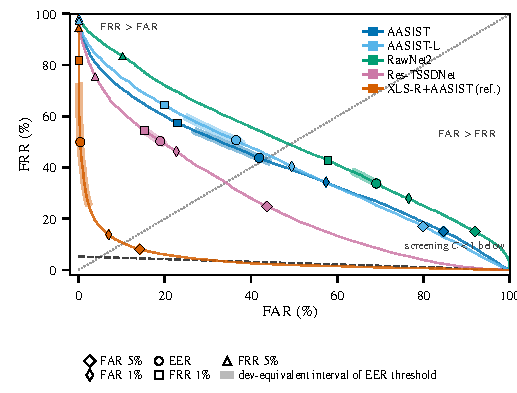
\includegraphics[width=\columnwidth]{fig_frr_far.pdf}
\caption{ITW: each curve is a model's FRR--FAR trade-off, markers are the five frozen thresholds, and the thick segment is the
interval of thresholds that tie with \(\tauE\) on dev (within one bona fide trial). Points above the diagonal put the error on
genuine speech, and screening \(C<1\) needs a point below the dashed line.}
\label{fig:frrfar}
\end{figure}

% src: revision/results/b_thresholds.json; revision/results/a_cluster.json
\emph{Determinacy.} Dev is nearly separable, so \(\tauE\) is pinned by few trials. For the reference, every threshold in
\([-3.38, +2.14]\) ties with \(\tauE\) on dev within one bona fide trial, and its ITW FRR runs from 25.1\% to 73.0\% over
that interval.

% src: revision/results/f_vad_stats_analysis.json; revision/results/f_vad_scores_analysis.json
\emph{Silence.} LA19 bona fide clips begin with a median 1.00\,s of silence against 0.38\,s for spoofs; ITW genuine clips
begin with 0.09\,s. Trimming both ends at test time raises the LA19-eval EER of all five models 6--34 fold, showing sensitivity to
the removed non-speech; this test-time intervention does not by itself isolate a learned silence shortcut; re-setting thresholds on trimmed dev lowers ITW FRR (9--38\,pp) but raises FAR (3--34\,pp) and moves ITW EER by
only \(-4.0\) to \(+3.1\)\,pp. Whether the cue in \emph{training} drives the ITW behaviour is R2-H3.

% src: revision/results/a5_cheapcheck.json; revision/results/e_cost.json
\emph{Checks for deployers.} Re-setting \(\tau\) from genuine channel speech alone restores FRR but accepts 88--99.9\% of
held-out spoofs for the primary models; and at \(\tauE\) on ITW a transferred detector beats the better trivial system only
in narrow windows of bona fide priors (none for RawNet2).

% src: results/phase_2_conversion_app/mlaad5/mlaad_report.json; results/phase_2_conversion_app/mlaad5/sample_rate_census.json; DEVIATIONS.md DEV-6.
\emph{Multilingual transfer, descriptive.} The original checkpoints were also scored on MLAAD \citep{mlaad24} paired with M-AILABS
bona fide speech (Table~\ref{tab:r1mlaad}). EER spans 24.8--37.7\%, and FAR exceeds FRR for four of five checkpoints at
\(\tauE\); Res-TSSDNet is the exception (FRR 60.78\%, FAR 18.42\%). Thus the FRR-dominant pattern on ITW and DF21 does
not extend to this surface. Every spoof file is native 22.05\,kHz, whereas 98.2\% of bona fide files are native
16\,kHz; resampling traces may contribute to separation, so these are not isolated language effects. These results
were known when round~2 was registered and remain descriptive.

% src: results/phase_2_conversion_app/mlaad5/mlaad_report.json; results/phase_2_conversion_app/mlaad5/sample_rate_census.json.
\begin{table}[!t]
\caption{Descriptive round-1 MLAAD/M-AILABS operating behaviour at \(\tauE\): rates in \%, TTG in pp.
Sample-rate confound: every spoof is native 22.05\,kHz and 98.2\% of bona fide speech is native 16\,kHz.}
\label{tab:r1mlaad}
\centering
\footnotesize
% src: results/phase_2_conversion_app/mlaad5/mlaad_report.json (models.*.fp32 only).
\begin{tabular}{@{}lrrrrr@{}}
\toprule
Model & EER & FRR & FAR & HTER & TTG \\
\midrule
AASIST & 27.21 & 6.49 & 60.06 & 33.28 & 7.11 \\
AASIST-L & 30.95 & 9.88 & 58.54 & 34.21 & 3.58 \\
RawNet2 & 27.58 & 4.52 & 60.22 & 32.37 & 5.03 \\
Res-TSSDNet & 37.69 & 60.78 & 18.42 & 39.60 & 2.02 \\
XLS-R+AASIST (ref.) & 24.80 & 18.75 & 31.49 & 25.12 & 0.38 \\
\bottomrule
\end{tabular}

\end{table}

\section{Round 2: Current Detectors, Retraining, Silence and Channels}
\label{sec:round2}
% src: results/round2/analysis/r2_registered.txt; results/round2/analysis/r2_explore.txt; DEVIATIONS.md DEV-9 amendment 5
Every registered round-2 score file was produced and passed its integrity review, so no detector, training run or
condition is missing from a registered test. The registered tests ran once, after the last of those files existed; the
exploratory analyses ran on the same files. The tables in this section are generated from the committed result files.
Unless stated otherwise, rates are at each model's frozen \(\tauE\), and intervals are speaker-cluster bootstrap
intervals.

\subsection{Gates and operating behaviour}
\label{sec:r2op}
% src: gen/r2_gates.tex; results/round2/gates.json; bib:wang25_asvspoof5_db; bib:pascu24_calibrated
All three reproduction gates pass (Table~\ref{tab:r2gates}). The ASVspoof~5 baseline reproduces its published development
EER (15.20\% against 15.2\%; \citealp{wang25_asvspoof5_db}), XLSR-Mamba's EER on verified DF21 is 1.62\% against 1.83\% for the
authors' released scores on the same 455,508 trials, and the train-plus-dev fit of Pascu's detector reaches 0.56\% on LA19
eval against the published 0.6\% \citep{pascu24_calibrated}.

% src: gen/r2_gates.tex; results/round2/gates.json
\begin{table}[!t]
\caption{Round-2 reproduction gates (EER, \%). Reference: the published value, or for XLSR-Mamba the authors' released
DF21 scores on the same trials. A gate passes within 15\% relative error.}
\label{tab:r2gates}
\centering
\footnotesize
\setlength{\tabcolsep}{4pt}
\gentab{r2_gates}
\end{table}

% src: gen/r2_operating.tex; results/round2/analysis/r2_explore.txt (E1); revision/results/b_thresholds.json
Table~\ref{tab:r2op} repeats the round-1 decomposition for the new detectors. The two LA19-trained self-supervised
detectors separate ITW far better than any round-1 primary model (EER 7.7\% for Pascu's detector and 9.2\% for
XLSR-Mamba, against 34--49\%), yet their development thresholds again reject much more genuine speech than they accept
spoofs. XLSR-Mamba rejects 41.5\% of genuine ITW clips and accepts 0.8\% of spoofs, so 57\% of its deployed HTER is
transfer (TTG 11.96\,pp [9.04, 16.79]); Pascu's detector rejects 19.9\% and accepts 2.5\% (TTG 3.59\,pp [1.64, 7.60],
32\%). Both also show FRR above FAR on verified DF21 (10.3\% against 0.7\%, and 4.9\% against 0.5\%), and most of their
small LA19-eval HTER is transfer (69\% and 76\%). The dev-equivalent interval matters as it did in round~1: across the
thresholds that tie with XLSR-Mamba's \(\tauE\) on dev, its ITW FRR runs from 19.4\% to 50.8\%, and from 17.7\% to
28.5\% for Pascu's detector.

% src: gen/r2_operating.tex; results/round2/analysis/r2_explore.txt (E1)
The ASVspoof~5 baseline behaves differently. Its EER is 26--37\% on every target, including its own evaluation set
(28.1\%), but its development threshold transfers within its own corpus (TTG 0.27\,pp on ASVspoof~5 eval) and to LA19
eval and DF21 (0.27 and 0.08\,pp). The direction of its error depends on the target: on LA19 eval it accepts 53.1\% of
spoofs and rejects 6.5\% of genuine clips, whereas on ITW it rejects 79.9\% of genuine speech and accepts 0.6\% of spoofs
(TTG 13.03\,pp), and on MLAAD-5 it rejects 69.9\%.

% src: gen/r2_operating.tex; results/round2/analysis/r2_explore.json (E1_E8_E10)
\begin{table*}[!t]
\caption{Round-2 detectors at the frozen \(\tauE\) (fp32, \%). Columns as in Table~\ref{tab:op}: HTER = oracle HTER + TTG
(pp, speaker-cluster 95\% CI, \(B=1000\)); Share = TTG/HTER (\%); the last column gives target FRR at the two ends of the
dev-equivalent interval. The ASVspoof~5 baseline takes its thresholds from ASVspoof~5 dev, the others from LA19 dev.}
\label{tab:r2op}
\centering
\footnotesize
\setlength{\tabcolsep}{4pt}
\resizebox{\textwidth}{!}{\gentab{r2_operating}}
\end{table*}

% src: gen/r2s_policies.tex; results/round2/analysis/r2_explore.json (E1_E8_E10)
The supplement gives every policy on every target (E1, E8, E10). A source APCER budget does not hold after transfer
either: at \(\tauA{5}\) the two self-supervised detectors accept 24.2\% and 23.5\% of ITW spoofs, so their BPCER of
2.3\% and 2.2\% there is not a BPCER at an APCER of 5\%; at the target threshold that does give 5\% APCER on ITW,
their BPCER is 11.0\% and 15.0\%. At \(\tauE\) on ITW, the break-even windows of all three new detectors contain the
forensic prior of 1/11 and exclude the screening prior of 0.95.

\subsection{Registered tests and reading rule}
\label{sec:r2tests}
% src: gen/r2_tests.tex; results/round2/analysis/r2_registered.txt
Table~\ref{tab:r2tests} gives the registered outcomes. \emph{R2-H1 is supported} (two of three detectors). For Pascu's
detector and XLSR-Mamba the strict FRR budget puts the error on genuine ITW speech (at \(\tauF{1}\), FRR 44.3\% and
86.1\% against FAR 0.5\% and 0.2\%) and the lenient FAR budget puts it on spoofs (at \(\tauA{5}\), FAR 24.2\% and 23.5\%
against FRR 2.3\% and 2.2\%), and all four tests reject after Holm correction. The ASVspoof~5 baseline meets the first
condition (+21.0\,pp [+5.1, +35.4]) but not the second: at \(\tauA{5}\) it rejects 99.8\% of genuine ITW speech and
accepts 0.1\% of spoofs. Its ITW scores lie almost entirely below its development thresholds, so for this detector the
target shift, not the policy, sets the direction of the error.

% src: gen/r2_tests.tex; results/round2/analysis/r2_registered.txt
\emph{R2-H2 is supported} (four of five runs). Retraining AASIST-L with seeds 1--5 gives LA19-eval TTGs at \(\tauE\) of
1.19 to 4.25\,pp. Four exceed the 1-pp margin after Holm correction; seed~1 (1.19\,pp [0.88, 1.55], \(p=.098\)) does
not. Transfer accounts for 43--80\% of each run's deployed HTER. The released checkpoint's LA19-eval gap (4.64\,pp) is
therefore not peculiar to one released file: under this recipe and its checkpoint-selection rule the gap recurs,
although its size varies more than threefold across seeds.

% src: gen/r2_tests.tex; results/round2/analysis/r2_registered.txt
\emph{R2-H3 indicates an operating-point effect.} Trimming raises development EER, as the manipulation check requires
(+2.00\,pp, \(p=.004\), the smallest \(p\) that 252 reassignments allow). Within the family, lower ITW FRR at \(\tauE\)
is supported (run means 16.8\% against 35.1\%, \(-18.33\)\,pp, \(p=.004\)), and lower ITW EER is not (the trimmed arm
is 1.99\,pp higher, \(p=.881\)). The registered reading is an operating-point effect without a discrimination gain.
Section~\ref{sec:r2seeds} shows that checkpoint selection contributes most of the FRR difference.

% src: gen/r2_tests.tex; results/round2/analysis/r2_registered.txt (R2-H4)
\emph{R2-H4 holds for four of the eight conditions.} Low-bitrate speech codecs push genuine speech below the development
threshold: Opus at 6\,kbps raises FRR by 40--69\,pp and AMR-NB at 4.75\,kbps by 77--92\,pp across the four primary
models, while FAR falls, so both conditions meet the rule for all four models. The phone impulse response raises FRR by
16--51\,pp (four of four). Opus at 24\,kbps also meets it for four of four, but through small shifts: FRR moves by at
most 1\,pp while FAR falls by 0.8--3.0\,pp. MP3 at 32\,kbps moves almost nothing (one of four). Additive noise splits the
models: AASIST and AASIST-L reject 41--74\,pp more genuine speech at 10 and 5\,dB SNR, whereas noise raises the FAR of
RawNet2 (by 2--22\,pp) and of Res-TSSDNet (by 27--31\,pp, at all three noise levels), so each noise level meets the rule
for two of four models only.

% src: gen/r2_tests.tex; results/round2/analysis/r2_registered.txt (R2-RL)
\emph{Reading rule.} The ASVspoof~5 baseline is discrimination-limited on ITW (EER 27.6\%). Pascu's detector and
XLSR-Mamba are transfer-limited: XLSR-Mamba by both criteria (transfer share 0.57; its dev-equivalent interval spans
31.4\,pp of ITW FRR), Pascu's detector by the span alone (10.8\,pp, share 0.32). No new detector is well-transferred. The
round-1 pattern of the self-supervised reference, strong ITW discrimination with a threshold far from the target
optimum, recurs for both new LA19-trained detectors.

% src: gen/r2_tests.tex; results/round2/analysis/r2_registered.json
\begin{table*}[!t]
\caption{Round-2 registered outcomes (speaker-cluster bootstrap, \(B=10{,}000\); exact permutation tests for R2-H3).
R2-H1: FRR\(-\)FAR at \(\tauF{1}\) / FAR\(-\)FRR at \(\tauA{5}\) on ITW (pp). R2-H2: LA19-eval TTG at \(\tauE\) per seed
(pp). R2-H3: trimmed minus untrimmed run means (pp; manipulation check, then the two tests of the family). R2-H4: models
meeting the rule per condition. \(^\ast\): rejected after Holm correction (R2-H1: both of the detector's tests
rejected). The reading rule is descriptive.}
\label{tab:r2tests}
\centering
\footnotesize
\setlength{\tabcolsep}{4pt}
\gentab{r2_tests}
\end{table*}

\subsection{Seed variation and silence-trimmed training}
\label{sec:r2seeds}
% src: gen/r2_seeds.tex; results/round2/analysis/r2_explore.txt (E2, E3); results/round2/gates.json
\emph{Seed variation (E2).} The five untrimmed runs come close to the released model's LA19-eval EER (1.07--1.63\%
against 0.99\%) but not to its ITW operating point (Table~\ref{tab:r2seeds}). The released checkpoint rejects more genuine
ITW speech than any retrained run (50.6\% against 24.7--43.8\%) and has a smaller ITW transfer gap than any (1.55 against
2.90--12.11\,pp), while ITW EER is similar (38.2--45.6\% against 44.5\%). The pipeline-check run (seed 1234, outside every
count) lies outside these ranges as well (LA19-eval TTG 6.18\,pp, ITW FRR 21.5\%). Our runs omit the author's
evaluation-based checkpoint step, so the released file comes from a slightly different procedure. An audit of one released
checkpoint therefore describes that file; the operating point of a recipe has to be read from several runs.

% src: gen/r2_seeds.tex; gen/r2s_last.tex; results/round2/analysis/r2_explore.txt (E3)
\emph{Checkpoint selection (E3).} The recipe's weight average absorbed 1 to 12 development-selected snapshots in the
untrimmed runs. Their last-epoch weights have similar LA19-eval EER (1.20--2.00\%) but larger transfer gaps: on LA19 eval
2.42--12.92\,pp (mean 7.59, against 2.69 for the averages), and on ITW a mean of 10.49\,pp against 6.51. The transfer gap
of R2-H2 is thus a property of the recipe together with its selection rule.

% src: gen/r2_seeds.tex; gen/r2s_last.tex; results/round2/runs/aasist_l_trim_s1/epochs.jsonl; bib:muller21_silence; bib:wang20_asvspoof2019
\emph{Silence-trimmed training.} Trimming silence from training, development and test audio keeps development EER low
(best epoch 1.72--2.31\%, scored model 2.06--3.33\%) but raises LA19-eval EER from 1.07--1.63\% to 21.3--23.7\%.
Without its leading and trailing non-speech, this recipe still separates the development attacks, which are the
training attacks \citep{wang20_asvspoof2019}, but no longer generalises to LA19's unseen attacks; the direction agrees
with \citet{muller21_silence}.

% src: gen/r2_seeds.tex; gen/r2s_last.tex; results/round2/analysis/r2_explore.json (E2_E3)
The registered R2-H3 comparison is not selection-free. The recipe averages only epochs whose development EER is at most
1\%, and no trimmed run reached that level, so each trimmed model is its last epoch, whereas each untrimmed model is an
average of selected snapshots. Comparing last-epoch weights in both arms (E3, exploratory) leaves a smaller difference:
ITW FRR at \(\tauE\) is 16.8\% for the trimmed and 23.4\% for the untrimmed runs (\(-6.6\)\,pp, against \(-18.3\)\,pp
as registered), lower for each of the five seeds by 1.2 to 12.4\,pp. About two thirds of the registered FRR difference
thus comes from checkpoint selection rather than from trimming. In both comparisons the lower FRR is paid for in FAR (ITW
FAR 86.5\% when trimmed, against 54.2\% for the averaged and 71.6\% for the last-epoch untrimmed models), and ITW EER does
not improve (+2.0 and +3.1\,pp). Trimming moves this recipe's ITW operating point; it does not make the recipe
discriminate ITW better.

% src: gen/r2_seeds.tex; results/round2/analysis/r2_explore.json (E2_E3); results/round2/gates.json
\begin{table*}[!t]
\caption{AASIST-L retrained (E2, E3) against the released checkpoint, at each run's \(\tauE\) from its own LA19 dev (rates
\%, TTG pp). SWA: snapshots in the recipe's weight average; best dev: lowest per-epoch dev EER; final dev: dev EER of the
scored model. Last-epoch weights: the run's weights after its final epoch (for the trimmed arm these are the scored
model). \(^\dagger\)Pipeline check, outside every test and mean.}
\label{tab:r2seeds}
\centering
\footnotesize
\setlength{\tabcolsep}{3pt}
\resizebox{\textwidth}{!}{\gentab{r2_seeds}}
\end{table*}

\subsection{Channels and shifted corpora}
\label{sec:r2chan}
% src: gen/r2_channels.tex; gen/r2s_channels.tex; results/round2/analysis/r2_explore.txt (E4)
\emph{Channel effects beyond the registered models (E4).} Table~\ref{tab:r2chan} adds the new detectors and the training
runs. The self-supervised detectors react much more to bandwidth-limiting codecs than to noise: Opus at 6\,kbps and
AMR-NB raise FRR by 92--99\,pp for Pascu's detector, XLSR-Mamba and the round-1 reference, and EnCodec raises it by 70
and 96\,pp for the two new ones, whereas 5-dB noise raises it by 5--17\,pp. The ASVspoof~5 baseline reacts least to these
codecs (+17 and +18\,pp) and most to noise (+21 to +37\,pp), and the phone impulse response raises its FAR (+12\,pp) rather
than its FRR. The untrimmed AASIST-L runs follow the released checkpoint (Opus 6\,kbps +49 against +69\,pp, AMR-NB +89
against +92\,pp). The trimmed runs react less to noise (+20 and +34\,pp at 10 and 5\,dB, against +52 and +74\,pp) but
much more to EnCodec (+39 against +5\,pp), and Opus 6\,kbps, AMR-NB and EnCodec lower their FAR by 26, 43 and 18\,pp.

% src: gen/r2_channels.tex; results/round2/analysis/r2_explore.json (E4)
\begin{table*}[!t]
\caption{Channel effects at \(\tauE\) on the 1,000-clip LA19-eval set (\(\Delta\)FRR/\(\Delta\)FAR in pp against the clean
copy, E4). Round-1 rows are the R2-H4 point estimates; run rows are means over seeds 1--5 (per run in the supplement).
EnCodec is the round-1 H5 condition; for the round-1 models it is reported in Table~\ref{tab:tests} (--).}
\label{tab:r2chan}
\centering
\footnotesize
\setlength{\tabcolsep}{4pt}
\resizebox{\textwidth}{!}{\gentab{r2_channels}}
\end{table*}

% src: gen/r2_mlaad.tex; gen/r2_operating.tex; results/round2/analysis/r2_explore.txt (E5); results/phase_2_conversion_app/mlaad5/sample_rate_census.json; DEVIATIONS.md DEV-9 amendment 5
\emph{MLAAD-5 (E5, descriptive).} The three new detectors have pooled EERs of 30--43\% on MLAAD-5
(Table~\ref{tab:r2mlaad}). The ASVspoof~5 baseline and Pascu's detector reject most genuine M-AILABS speech in every
language (FRR 56--78\% and 79--94\%), whereas XLSR-Mamba accepts 42--65\% of spoofs at FRR 1--18\%. Pascu's scores come
from the single rerun allowed by amendment~5, which repeated two 186-sample spoofs to 400 samples and scored all 494,853
trials. Every spoof file is native 22.05\,kHz and 98.2\% of bona fide files are native 16\,kHz, so these rates mix
language, synthesis system and sample-rate history and isolate none of them.

% src: gen/r2_mlaad.tex; results/round2/analysis/r2_explore.json (E5); results/phase_2_conversion_app/mlaad5/sample_rate_census.json
\begin{table}[!t]
\caption{Round-2 detectors on MLAAD-5 by language: FRR/FAR (\%) at \(\tauE\) (E5, descriptive). Sample-rate confound:
every spoof is native 22.05\,kHz and 98.2\% of bona fide speech native 16\,kHz.}
\label{tab:r2mlaad}
\centering
\footnotesize
\gentab{r2_mlaad}
\end{table}

% src: gen/r2_as5.tex; results/round2/analysis/r2_explore.txt (E6); bib:wang25_asvspoof5_db
\emph{ASVspoof~5 by condition (E6).} On its own evaluation set the baseline's error depends on the channel
(Table~\ref{tab:r2as5}). Its threshold transfers to the codec-free subset C00 (EER 22.4\%, TTG 0.03\,pp) and to the
wideband codecs C01--C07 (TTG at most 0.98\,pp), but the narrowband conditions C08--C11, coded at 8\,kHz
\citep{wang25_asvspoof5_db}, raise FRR to 40.6--65.9\% and the transfer gap to 3.06--5.45\,pp. This is the pattern of
round~1 and R2-H4 inside one corpus: band-limited coding pushes genuine speech below a development threshold. Unlike LA19,
ASVspoof~5 shows no class difference in leading silence: the median is 0.03\,s for bona fide clips and 0.02--0.03\,s for
spoofs in both development and evaluation data.

% src: gen/r2_as5.tex; results/round2/analysis/r2_explore.json (E6)
\begin{table}[!t]
\caption{The ASVspoof~5 baseline on ASVspoof~5 eval by codec condition at \(\tauE\) from ASVspoof~5 dev (E6): rates \%,
TTG pp. C00: no codec; C01--C07: 16-kHz codecs; C08--C11: 8-kHz conditions.}
\label{tab:r2as5}
\centering
\footnotesize
\gentab{r2_as5}
\end{table}

\subsection{Review policies and calibration across priors}
\label{sec:r2review}
% src: gen/r2_threezone.tex; gen/r2s_budgets.tex; results/round2/analysis/r2_explore.txt (E7)
\emph{Three-zone review (E7).} A review band that holds 10\% of development traffic does not hold 10\% of ITW traffic
(Table~\ref{tab:r2three}). For every LA19-trained detector, ITW scores crowd into the band: it sends 63.1--88.8\% of ITW
clips, and 77.4--98.2\% of genuine ones, to review, and the automatic decisions that remain reject 1.8--22.4\% of genuine
clips and accept almost no spoofs. The ASVspoof~5 baseline keeps its review share near budget (13.7\%) only because most
genuine ITW scores fall below the band, so it auto-rejects 68.3\% of genuine clips. Re-anchoring the band on the unlabelled
target scores restores the 10\% budget by construction but moves the errors into the automatic decisions: 12.9--72.2\% of
genuine ITW clips are then rejected without review. With target labels, the same budget would auto-reject 4.6\% and 4.8\%
of genuine clips for XLSR-Mamba and Pascu's detector. The error-budget rule, which reviews the scores between \(\tauF{1}\)
and \(\tauA{1}\), collapses to a single threshold for every LA19-trained detector, because the two thresholds cross on
nearly separable development data; only the ASVspoof~5 baseline keeps a band, which then holds 45.3\% of ITW. A review
budget, like a threshold, is a property of the development distribution.

% src: gen/r2_threezone.tex; results/round2/analysis/r2_explore.json (E7)
\begin{table*}[!t]
\caption{Three-zone review on ITW (E7): a band holding 10\% of pooled dev scores, centred in rank on \(\tauE\), in \% of
ITW clips. Review: all clips sent to review; Gen.\ in review: genuine clips sent to review; Gen.\ rej.: genuine clips
rejected automatically; Spoof acc.: spoofs accepted automatically. Label-free: the same 10\% re-anchored on the
unlabelled ITW scores. Error-budget rule: review between \(\tauF{1}\) and \(\tauA{1}\). Other targets and budgets of 5\%
and 20\% are in the supplement.}
\label{tab:r2three}
\centering
\footnotesize
\setlength{\tabcolsep}{4pt}
\resizebox{\textwidth}{!}{\gentab{r2_threezone}}
\end{table*}

% src: gen/r2_calibration.tex; gen/r2s_calibration.tex; results/round2/analysis/r2_explore.txt (E9); DEVIATIONS.md DEV-9 amendment 2
\emph{Calibration across priors (E9).} A logistic calibration fitted on source development scores does not remove the
transfer loss (Table~\ref{tab:r2cal}). Actual cost exceeds minimum cost on every target. At equal priors on ITW the excess
is largest for the self-supervised detectors (0.44 against 0.18 for XLSR-Mamba, 0.53 against 0.20 for the round-1
reference, 0.23 against 0.15 for Pascu's detector), whereas the round-1 primary models come close to their minimum because
the minimum itself is near 1 (0.68--0.92). RawNet2 on ITW (1.02) and Pascu's detector on MLAAD-5 (1.09) do worse than the
better trivial system even after calibration. At a bona fide prior with logit 2 (about 0.88), every detector costs more on
ITW than accepting everything (1.18--3.60), although the minimum stays below 1 for the self-supervised ones (0.39--0.58).
The gap between actual and minimum cost is the cost-domain counterpart of TTG, and a calibration fitted on source data
inherits it.

% src: gen/r2_calibration.tex; results/round2/analysis/r2_explore.json (E9)
\begin{table}[!t]
\caption{Actual/minimum normalised cost at equal priors after a logistic calibration fitted on source dev (E9; 1 = the
better trivial system). The supplement gives the bona fide priors with logit \(-2\) and \(+2\).}
\label{tab:r2cal}
\centering
\footnotesize
\setlength{\tabcolsep}{4pt}
\gentab{r2_calibration}
\end{table}

% src: PREREGISTRATION.md; PREREGISTRATION_ROUND2.md; DEVIATIONS.md DEV-8; revision/paper/main.tex
\section{Discussion and Limitations}
\label{sec:discussion}
\subsection{What a transferred operating point establishes}
The round-1 audit distinguishes a detector that orders target scores poorly from one whose source threshold sits
poorly on otherwise informative scores. Both can produce a high deployed error, but they suggest different responses.
Changing a threshold cannot repair poor discrimination. Conversely, selecting a detector solely by target-oracle EER
does not address how a source threshold will behave on genuine target speech. The false-rejection and
false-acceptance decomposition is therefore needed alongside HTER and its transfer gap.

% src: PREREGISTRATION.md; PREREGISTRATION_ROUND2.md; DEVIATIONS.md DEV-8; revision/paper/main.tex
The reporting card is intended to make these distinctions inspectable. It requires the threshold source and
estimator, the application policy, the target error components and an oracle reference computed only for analysis.
The target oracle is not an available deployment policy unless labelled target data can actually be collected.
Similarly, the genuine-speech-only threshold reset in round~1 measures a tradeoff: restoring a rejection budget
does not establish a useful spoof detector. A workflow that uses the scores for review must assess review load and
automatic errors separately; Section~\ref{sec:r2review} shows that a review budget designed on development data is not
kept after transfer.

\subsection{What carries over from round 1}
% src: results/round2/analysis/r2_registered.txt; results/round2/analysis/r2_explore.txt; gen/r2_operating.tex; gen/r2s_last.tex
Round~2 tested the round-1 observations on new scores, and four of them carry over. First, the dominant error on a
shifted target follows the operating policy (R2-H1, two of three detectors): a strict false-rejection budget puts the
error on genuine ITW speech, and a lenient false-acceptance budget puts it on spoofs. The exception, the ASVspoof~5
baseline, rejects almost all genuine ITW speech even at its most lenient registered threshold; there the target shift
overrides the policy. Second, the transfer gap on LA19 eval belongs to the AASIST-L recipe and its checkpoint selection,
not only to the released file (R2-H2), although its size depends on the seed and on the selection rule. Third, better
discrimination did not bring better transfer: both new LA19-trained detectors discriminate ITW far better than the
round-1 primary models and are transfer-limited, as the round-1 reference was. Fourth, band-limiting and low-bitrate
channels raise false rejection: R2-H4 holds for both low-bitrate speech codecs and the phone impulse response, and the
narrowband conditions of ASVspoof~5 show the same pattern, whereas the effect of additive noise depends on the model.

% src: results/round2/analysis/r2_registered.txt; gen/r2_seeds.tex; gen/r2s_last.tex
Two observations do not carry over in the form that round~1 suggested. Removing silence from training lowers ITW false
rejection at the development threshold, but about two thirds of that reduction comes from checkpoint selection, FAR
rises, and ITW discrimination does not improve. The silence cue thus helps explain where this recipe's ITW operating
point falls, not why the recipe fails to discriminate ITW. And a released checkpoint's ITW operating point is not the
recipe's: the released AASIST-L rejects more genuine ITW speech than any of its retrained counterparts.

% src: results/round2/analysis/r2_registered.txt; results/round2/analysis/r2_explore.txt
For reporting, round~2 strengthens three items of the card (Table~\ref{tab:card}). The threshold policy and its source
belong with every rate, because they decide which error dominates. The dev-equivalent interval belongs with every
\(\tauE\) set on nearly separable development data: across that interval, XLSR-Mamba's ITW FRR spans 31.4\,pp. And a
review policy has to be assessed by its review share and its automatic errors on the target: a budget set on development
data is not kept after transfer, and re-anchoring it without labels keeps the budget only by automating errors.

\subsection{Scope of inference}
The released-checkpoint audit inherits each author's training, augmentation and model-selection choices. Its roster
was selected for a broader deployment project rather than sampled from the population of speech detectors. Related
models share a lineage, and the self-supervised reference enters no primary-model hypothesis count. The registered
extension broadens this evidence but still retrains only AASIST-L. An observation across its seeds supports a
statement about that recipe under the recorded training and selection rules; it does not identify an architecture
effect across independently trained detector families.

% src: PREREGISTRATION.md; PREREGISTRATION_ROUND2.md; DEVIATIONS.md DEV-8; revision/paper/main.tex
The ASVspoof~5 detector differs from LA19-trained detectors in more than silence handling, including its training
corpus. Its training audio was not subject to the development/evaluation post-processing
\citep{wang25_asvspoof5_db}. It therefore cannot isolate a causal effect of removing silence during training. The
trimmed and untrimmed AASIST-L arms provide the registered intervention. Even there, the intervention changes both
training and threshold-source preprocessing, and the recipe's weight-averaging eligibility did differ between arms: no
trimmed run reached the averaging threshold. The selection-free last-epoch comparison separates most of that difference,
but it is exploratory, and five runs per arm limit any permutation test to \(p\geq1/252\). Test-time trimming alone, as
in round~1, can expose reliance on a cue but cannot establish why a detector learned it.

% src: PREREGISTRATION.md; PREREGISTRATION_ROUND2.md; DEVIATIONS.md DEV-8; revision/paper/main.tex
\subsection{Data, dependence and ecological validity}
ITW is a community-exposed benchmark, not a prospective sample of previously unseen deployment traffic
\citep{muller22_in_the_wild}. Its metadata identify speakers but not source recordings. Speaker-cluster inference
accounts for within-speaker dependence under the recorded labels; recording-specific effects and dependence that
crosses speaker labels cannot be separated from those labels. The disagreement between clip-level and
speaker-level H2 inference is part of the audit's evidence, rather than a reason to substitute one registered
result for the other. The exploratory H1 and H4 comparisons likewise rest on few distinct models, so multiple
model-policy points do not create independent model replications.

% src: PREREGISTRATION.md; PREREGISTRATION_ROUND2.md; DEVIATIONS.md DEV-8; revision/paper/main.tex
The DF21 analysis uses the documented integrity-verified evaluation surface. Excluding audio that cannot reproduce
its own encoded checksum changes the evaluated population, and the clean-surface sensitivity analysis does not
recover the omitted trials. Our DF21 measurements must therefore be identified by their surface and should not be
equated with published measurements on a different subset or decode. The checksum verification and decoder
amendment are reproducibility requirements, not an estimate that the excluded trials are harmless.

% src: PREREGISTRATION.md; PREREGISTRATION_ROUND2.md; DEVIATIONS.md DEV-8; revision/paper/main.tex
MLAAD paired with M-AILABS adds languages and synthesis systems but also a class-associated sample-rate difference.
Resampling traces may contribute to separation, so a pooled or language-specific error rate cannot be interpreted
as an isolated language effect. The original round-1 MLAAD scores were already known when the extension was
registered; their reporting remains descriptive. Bona fide speaker and spoof-system clustering measures the
available dependence structure, not independence of every utterance.

% src: PREREGISTRATION.md; PREREGISTRATION_ROUND2.md; DEVIATIONS.md DEV-8; revision/paper/main.tex
The stress experiments preserve clip identity and isolate specified transformations. A codec reconstruction of
genuine speech retains its genuine label under this channel-use interpretation; codec-based generation can have
another role in synthesis benchmarks \citep{wu24_codecfake,wang25_asvspoof5_db,xiao26_resynth}. The experiments cover
single-pass digital transformations and impulse-response convolution. They do not reproduce an entire live
transmission chain, a physical re-recording campaign or an adaptive adversary. Desktop scoring does not establish
on-device numerical parity, latency or energy performance.

% src: PREREGISTRATION.md; PREREGISTRATION_ROUND2.md; DEVIATIONS.md DEV-8; revision/paper/main.tex
\subsection{Registration and reporting boundaries}
The tagged registration and deviation log provide a version-controlled chronology rather than an independently
deposited registration. Some original amendments followed pilot or reproduction observations, and the speaker-level
sensitivity analyses were requested after the round-1 results were known. The manuscript reports that chronology,
preserves the original clip-level outcomes and labels the added analyses as exploratory. Round~2 was designed in
response to those observations; its registration protects the later tests from adaptation to its own scores,
without making the original observations unknown at design time.

Our costs are explicit evaluation scenarios, not measured operational priors or monetary losses. A review policy
does not model reviewer accuracy, staffing, delay or consent requirements for collecting genuine channel speech.
The audit characterizes detector limitations and the evidence needed to assess them; it does not certify an
authenticity decision for a particular speaker or forensic case.


\section{Conclusion}
\label{sec:conclusion}
% src: results/round2/analysis/r2_registered.txt; results/round2/analysis/r2_explore.txt; revision/paper/main.tex
A countermeasure is thresholded once, on development data, and deployed elsewhere. Across two registered rounds, eight
detectors and eleven training runs, the threshold decided much of what the detectors did after transfer: which error
dominated, how much of the deployed error a better threshold would have removed, how much traffic a review band
received, and how far a calibrated cost stayed from its minimum. The equal error rate on the target hides all four,
because it chooses the threshold with the target labels. The detectors that ordered In-the-Wild scores best lost a much
larger share of their deployed error to the threshold than the round-1 primary models did: both current LA19-trained
self-supervised detectors, like the round-1 reference, were limited by transfer rather than by discrimination.

The registered extension also qualified two round-1 readings. The transfer gap of a released checkpoint recurred across
retraining, but its size depended on the seed and on the checkpoint-selection rule, and the released file's operating
point lay outside the range of its retrained counterparts. Removing the silence cue from training moved the operating
point rather than improving discrimination, and much of that movement came from checkpoint selection. Claims about a
recipe therefore need several runs and a stated selection rule, and claims about a cue need a selection-free comparison.

We recommend that speech deepfake evaluations report, for every threshold policy and target, the false-rejection and
false-acceptance rates at the shipped threshold, the split of HTER into oracle HTER and TTG with speaker-level
intervals, the range of thresholds that tie on development data, and, where scores route traffic to review, the review
share and automatic errors on the target. A separate deployment study will apply the same protocol to converted and
quantized models on mobile devices.

\section*{CRediT authorship contribution statement}
\todo{Authors: confirm the author list and assign the applicable CRediT roles to each author.}

\section*{Declaration of competing interest}
\todo{Authors: provide the competing-interest declaration after confirming any financial or personal relationships.}

\section*{Funding}
\todo{Authors: provide funding bodies and grant identifiers, or confirm that no specific funding supported this work.}

\section*{Data availability}
The study uses the public speech corpora cited in the manuscript, subject to their respective access conditions and
licences. The reproducibility package comprises the permitted utterance-level score files, frozen thresholds,
manifests, registration snapshots, deviation log and analysis code. Source audio and restricted checkpoints are
obtained from their original providers. \todo{Authors: insert a stable public repository or archive URL, confirm its
contents and licensing, and identify any access restrictions before submission.}

\section*{Declaration of generative AI and AI-assisted technologies in the manuscript preparation process}
During preparation of this manuscript, the authors used OpenAI Codex to assist with drafting and revising text,
manuscript formatting, citation checks and automated numerical-claim checks.
\todo{Authors: verify and complete the tool inventory, including any earlier Claude use, and review the final text,
references and analyses. The submitted statement must accurately describe the assistance used and affirm author
responsibility after that review has occurred.}


\bibliographystyle{elsarticle-harv}
\bibliography{refs}

\end{document}
